\documentclass[tikz,border=10pt]{standalone}
\usepackage{tikz}
\usetikzlibrary{arrows.meta,positioning,shapes,calc}

\begin{document}
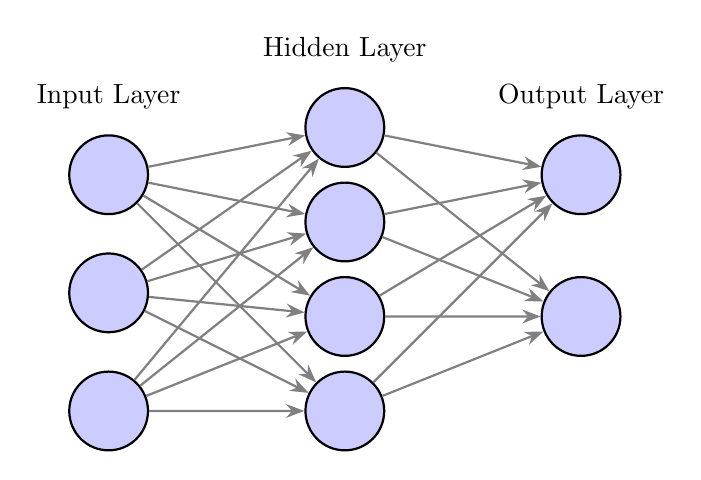
\begin{tikzpicture}[
    neuron/.style={circle, draw, thick, minimum size=1cm, fill=blue!20},
    layer/.style={rectangle, draw=none},
    arrow/.style={-Stealth, thick}
]

% Input layer
\foreach \i in {1,2,3} {
    \node[neuron] (input\i) at (0, -\i*1.5) {};
}
\node[above=0.2cm of input1] {Input Layer};

% Hidden layer
\foreach \i in {1,2,3,4} {
    \node[neuron] (hidden\i) at (3, -\i*1.2 + 0.3) {};
}
\node[above=0.2cm of hidden1] {Hidden Layer};

% Output layer
\foreach \i in {1,2} {
    \node[neuron] (output\i) at (6, -\i*1.8 + 0.3) {};
}
\node[above=0.2cm of output1] {Output Layer};

% Connections
\foreach \i in {1,2,3} {
    \foreach \j in {1,2,3,4} {
        \draw[arrow, gray] (input\i) -- (hidden\j);
    }
}

\foreach \i in {1,2,3,4} {
    \foreach \j in {1,2} {
        \draw[arrow, gray] (hidden\i) -- (output\j);
    }
}

\end{tikzpicture}
\end{document}
